
\section{Formulation}

We begin by looking at a Light Curtain only problem of adaptively discovering the depth of a scene. We wouldn't know the path along the rays/pixels on which an object may lie/intersect, hence we choose to go with a sampling based approach. We treat each ray as initially having either a uniform distribution, or a gaussian with a large variance in the center, and we attempt to formulate our problem with a Recursive Bayesian update approach.

\subsection{Representation}

\smallskip
Our state space is represented as a tensor of some fixed resolution [320x240] with each pixel in image $I$ encoding the depth value $\mathbf{d}(u,v)$ as a bernoulli distribution $P(\mathbf{d}(u,v))$. $D_{c}$ represents the list of depths quantizing the space of each pixel defined within $(d_{min}, d_{max})$ of some fixed size $N$ [64], resulting in a Depth Probability Volume (DPV) tensor of size [64, 240, 320]
\begin{align}
   D_{c}=\left\{ d_{0}...d_{n}\right\} \quad d_{i}=d_{min}+(d_{max}-d_{min})*t 
   \label{eq:d_candi}
   \\
   P(\mathbf{d}(u,v))=I(u,v)
   \nonumber\\
   \sum_{d}\left(P(\mathbf{d}(u,v))\right)=1\qquad \mathbb{E}[P(\mathbf{d}(u,v))]=\mathbf{d}(u,v)
   \label{eq:depth_dist}
   %\vspace{-.1in}
\end{align}

While an ideal sensor could choose plan a path to sample in the full 3D volume, our Light Curtain device only has control over a collapsed XZ  space. Hence, we select a subset of rays that correspond to a plane that we wish to sample, and generate an Uncertainty Field (UF) as follows:
\begin{align}
   P(\mathbf{d}(u))=\frac{\sum_{u,v}P(\mathbf{d}{(u,v)}).\boldsymbol{1}}{\sum_{u,v}\boldsymbol{1}}
   \nonumber \\
   \;where\;h_{min}>\mathbb{E}[P(\mathbf{d}(u,v))]>h_{max}
   \label{eq:collapse}
   %\vspace{-.1in}
\end{align}

\begin{figure}[h]
   \centering
   \begin{minipage}{0.5\textwidth}
       \centering
       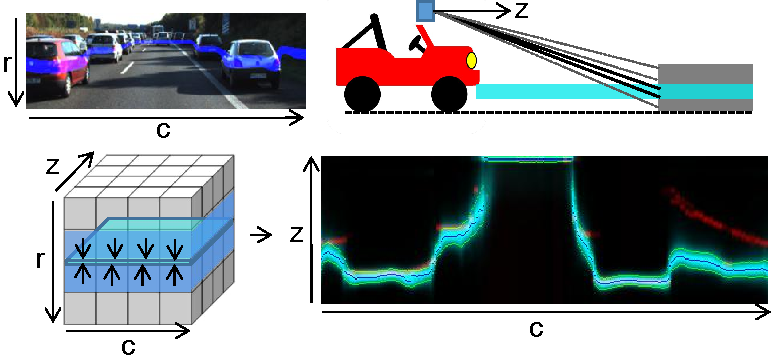
\includegraphics[width=1.0\textwidth]{figures/bev.pdf}
   \end{minipage}\hfill
   \centering
   \caption{Our state space consisting of a Depth Probability Volume (DPV) its corrsp Bird's Eye Uncertainty Field (UF)}
\end{figure}

\subsection{Curtain Planning}

With the Uncertainty Field (UF) extracted from the state space, we can use this to figure out where to place light curtains. We build upon prior work solving Light Curtain placement as a Constraint Optimization and Dynamic Programming problem. A single light curtain placement is defined by a set of $T$ control points $\{\X_t\}_{t=1}^T$. We wish to maximize the objective $J(\X_1, \dots, \X_T) = \sum_{t=1}^T UF(\X_t)$ where $UF(\X)$ is the uncertaintiy field probabilies at the anchor location of $\X$.

The control points $\{\X_t\}_{t=1}^T$, where each $\X_t$ lies on the the camera ray $\R_t$, must be chosen to satisfy the physical constraints of the light curtain device: $|\theta(\X_{t+1}) - \theta(\X_t)| \leq \Delta \theta_\text{max}$ with $\theta_\text{max}$ being the maximum angular velocity of the Galvomirror. The problem is also discretized such that $\X_{t} \in D_c\ $ and also lies along $\R_t$
\begin{align}
    &\arg \max_{\{\X_t\}_{t=1}^T} \sum_{t=1}^T UF(\X_t) \qquad \text{where}\ \X_t \in D_c\ \nonumber\\
    &\text{subject to}\ |\theta(\X_{t+1}) - \theta(\X_t)| \leq \dtmax,\ \forall 1 \leq t < T
    \label{eq:constraint}
\end{align}

\begin{figure}[h]
   \centering
   \begin{minipage}{0.5\textwidth}
       \centering
       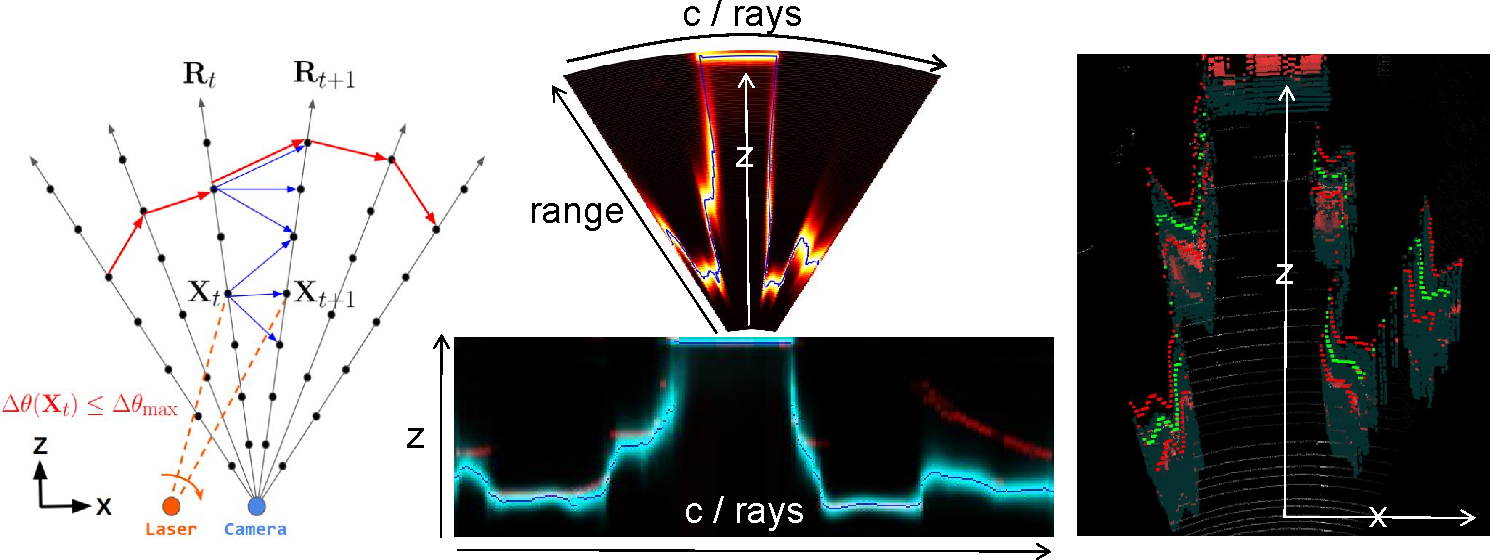
\includegraphics[width=1.0\textwidth]{figures/planner.pdf}
   \end{minipage}\hfill
   \centering
   \caption{Left: Light Curtain constraint graph subject to max angular velocity of Galvomirror. Right: Placing an optimal curtain along the highest probability region per column of rays}
\end{figure}

In the figure above, we have placed a single curtain along the highest probability region per column of rays, but ideally, we should place more curtains spanning the uncertaintiy of those distributions. To do this, we generate corresponding entropy fields $H(\X)_{i}$ to be fed to the planner from $UF(\X)$ based on two approaches: $m0$ attempts to normalize each ray's distribution $P(\mathbf{d}(u))$ and warp the distribution such that a selected span from the mean is maximized. $m1$ attempts to sample a point on the ray given $P(\mathbf{d}(u))$. 

\begin{figure}[h]
   \centering
   \begin{minipage}{0.5\textwidth}
       \centering
       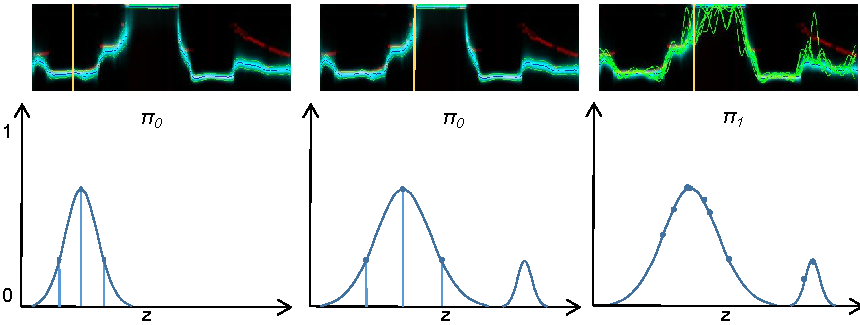
\includegraphics[width=1.0\textwidth]{figures/fields.pdf}
   \end{minipage}\hfill
   \centering
   \caption{We look at a depth distribution of one of the rays in UF (yellow line), and figure out where additional curtains (blue points) can be placed such as to maximize information gained. Observe that $m1$ is able to handle multimodal distributions}
   \label{fig:m0m1}
\end{figure}

As seen in Fig. ~\ref{fig:m0m1}, strategy $m0$ is able to generate fields that adaptively place additional curtains around a consistent span around the mean, but is unable to do so in cases of multimodal distributions. $m1$ on the other hand is able to place a curtain around the 2nd modality, albeit with a lower probability. The inconsistency from ray to ray in $m1$ however, may be impossible to image due to it exceeding the acceleration bounds, hence a spline fit is used with control points every 5 to 10 rays, resulting in an imagable but non-flat curtain placement. We see the effects of both in later experiments.

\subsection{Observation Model}

We now have returns from curtains $\mathbf{C}$ with each $\mathbf{C}_{i}$ containing $[x,y,z,i]$, the 3D position and intensity value in the same spatial resolution as $I$, planned based on a particular policy, conditioned on our prior distribution $P(\mathbf{d}_{t})$ at time $t$. We need to convert $\mathbf{C}_{i}$ into a likelihood distribution $P(\mathbf{c}_{t}|\mathbf{d}_{t})$, such that this Hidden Markov Model representation and sum of log likelihoods holds true:
\small
\begin{align}
   P\left(\mathbf{d}_{0},...,\mathbf{d}_{T},\mathbf{c}_{1},...,\mathbf{c}_{T}\right)= 
   P\left(\mathbf{d}_{0}\right)\mathbf{\mathbf{\prod}_{\mathrm{t=1}}^{\mathrm{T}}}P\left(\mathbf{c}_{t}|\mathbf{d}_{t}\right)P\left(\mathbf{d}_{t}|\mathbf{d}_{t-1}\right) \nonumber\\
   \log\left(P\left(\mathbf{c}_{t}|\mathbf{d}_{t}\right)\right)=\stackrel[i=0]{n}{\sum}\left(\log\left(P\left(\mathbf{c_{\mathit{i}}}_{t}|\mathbf{d}_{t}\right)\right)\right)
   \label{eq:hmm}
\end{align}
\normalsize

We represent $P\left(\mathbf{c_{\mathit{i}}}_{t}|\mathbf{d}_{t}\right)$ as a linear combination of a gaussian and a uniform distribution, where $\sigma$ is a function of the thickness of the light curtain as described earlier where $t\in[-1..1]$. $t$ is a function of the intensity value $i$, based on two possible profiles where $z$ either takes a value of 0.5 or 1.0, and $m$ is some control factor we tune:

\small
\begin{align}
   P\left(\mathbf{c_{\mathit{i}}}_{t}|\mathbf{d}_{t}\right)=\frac{\mathcal{N}\left(D_{c},\mu_{c},\sigma_{c}\right)\left(t\right)+U\left(D_{c}\right)(1-t)}{\sum\left(\mathcal{N}\left(D_{c},\mu_{c},\sigma_{c}\right)\left(t\right)+U\left(D_{c}\right)(1-t)\right)} \\
   t=\left(\frac{-1}{\left(z\right)+\left(mi\right)}\right)+1
   \label{eq:dist}
\end{align}
\normalsize

\begin{figure}[h]
   \centering
   \begin{minipage}{0.5\textwidth}
       \centering
       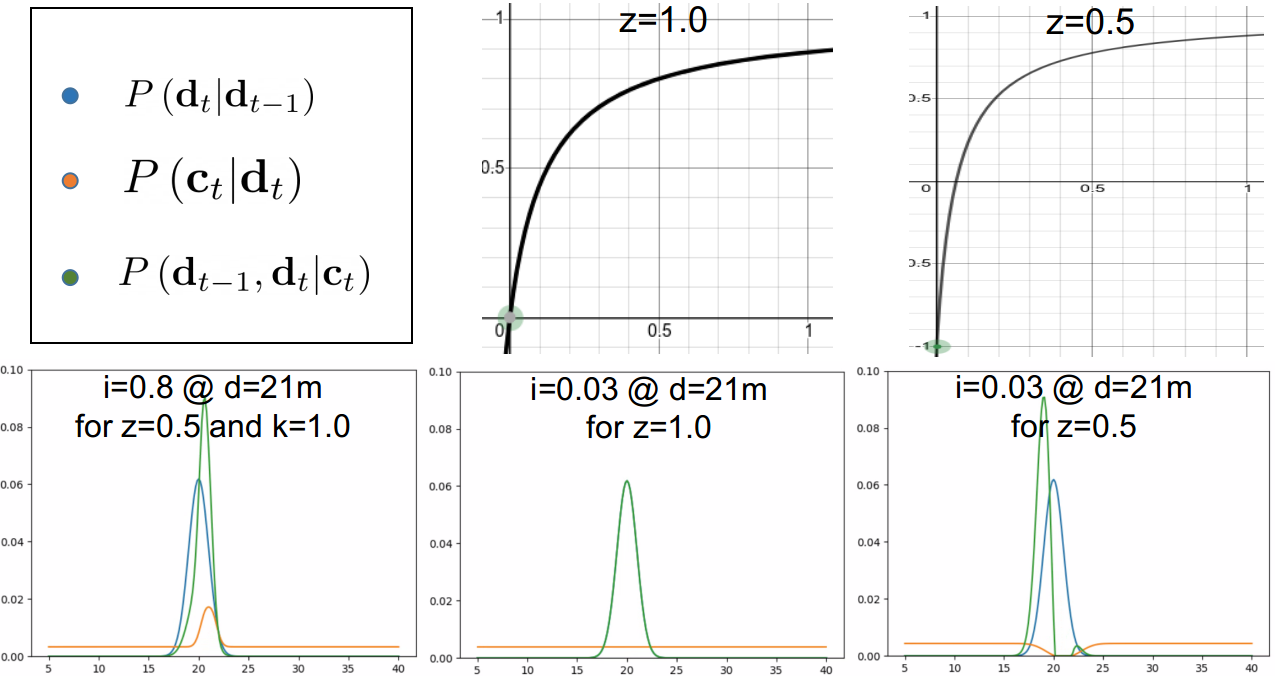
\includegraphics[width=1.0\textwidth]{figures/graphs.png}
   \end{minipage}\hfill
   \centering
   \caption{The effect on the posterior when getting a close to 0 intensity return from the Light Curtain when $z$ is either 1.0 or 0.5}
   \label{fig:updatemodel}
\end{figure}

As seen in Fig. ~\ref{fig:updatemodel}, as the intensity of the light curtain varies from 0 to 1 on the $x$ axis, we vary the value of $t$ on the $y$ axis. When $z$ is 0.5, low intensity returns (eg. < 0.1) results in a negative $t$ value. This means that when the intensity is high, a higher return results in a larger peak probability for both cases when $z$ is 1.0 or 0.5. But when the intensity is low or close to 0, $z=1.0$ causes $P\left(\mathbf{c}_{t}|\mathbf{d}_{t}\right)$ to tend to a uniform distribution, but $z=0.5$ to tend to an inverted gaussian. With this case, the rationale is that having no return at a location doesn't mean that we have derived no information at all, but rather, we know that this particular location is less likely to have an object and the rest of the the locations along the ray are equally uncertain/uniform. We show in experiments that this results in significantly faster convergence.